% Name: Fourier series
% Description: A square wave and its Fourier partial sums with one, two, and five terms, closing in on the jumps with the overshoot of the Gibbs phenomenon.
% Tags: Fourier series, square wave, partial sums, Gibbs phenomenon

\usepackage{pgfplots}
\pgfplotsset{compat=1.18}

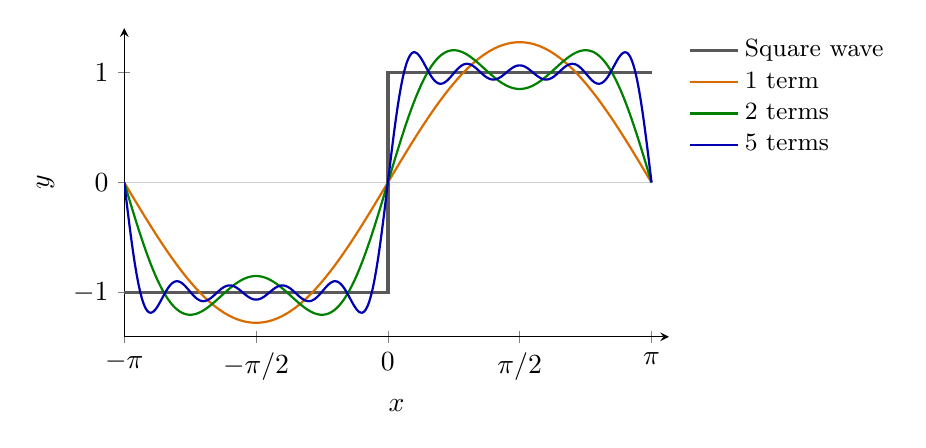
\begin{tikzpicture}
  \begin{axis}[
    width=8.5cm, height=5.5cm, axis lines=left, domain=-pi:pi, samples=300,
    xmin=-3.1416, xmax=3.35, ymin=-1.4, ymax=1.4, xlabel=$x$, ylabel=$y$,
    xtick={-3.1416,-1.5708,0,1.5708,3.1416}, xticklabels={$-\pi$,$-\pi/2$,$0$,$\pi/2$,$\pi$}, ytick={-1,0,1},
    legend style={at={(1.02,1)}, anchor=north west, draw=none, font=\small}, legend cell align=left,
  ]
    \draw[gray!40] (axis cs:-3.1416,0) -- (axis cs:3.1416,0);
    \addplot[gray!70!black, very thick, const plot, samples=3] coordinates {(-3.1416,-1) (0,1) (3.1416,1)};
    % S_n(x) = (4/pi) * sum over odd k up to 2n - 1 of sin(kx)/k.
    \addplot[orange!85!black, thick] {4/pi*sin(deg(x))};
    \addplot[green!50!black, thick] {4/pi*(sin(deg(x)) + sin(deg(3*x))/3)};
    \addplot[blue!70!black, thick] {4/pi*(sin(deg(x)) + sin(deg(3*x))/3 + sin(deg(5*x))/5 + sin(deg(7*x))/7 + sin(deg(9*x))/9)};
    \legend{Square wave, 1 term, 2 terms, 5 terms}
  \end{axis}
\end{tikzpicture}
